% Model report generated by SolverMapp.
% Compile with pdflatex (twice, for the equation and algorithm references).
\documentclass[11pt,a4paper]{article}
\usepackage[T1]{fontenc}
\usepackage[utf8]{inputenc}
\usepackage{lmodern}
\usepackage{amsmath,amssymb}
\usepackage{booktabs,longtable}
\usepackage{siunitx}
\usepackage{algorithm}
\usepackage{algpseudocode}
\usepackage{tikz}
\usetikzlibrary{positioning,shapes.geometric,shapes.misc,arrows.meta}
\usepackage{adjustbox}
\usepackage[hidelinks]{hyperref}

\title{Pipe flow: viscosity function, laminar / turbulent switch}
\author{}
\date{\today}

\begin{document}
\maketitle

The model consists of 5 equations in 13 variables: 9 inputs, 0 state variables, 3 intermediate variables and 1 output. It is solved in 4 steps (Algorithm~\ref{alg:solution}).

\section{Nomenclature}
\begin{longtable}{@{}l p{0.48\linewidth} l l@{}}
  \toprule
  Symbol & Description & Unit & Value \\
  \midrule
  \endhead
  \bottomrule
  \endfoot
  \multicolumn{4}{@{}l}{\textit{Inputs}} \\
  $\mu_0$ & Viscosity at T\_0 & \si{Pa.s} & \num{1e-3} \\
  $B$ & Viscosity constant & \si{K} & \num{1800} \\
  $T_0$ & Reference temperature & \si{K} & \num{293} \\
  $\rho$ & Density & \si{kg/m^{3}} & \num{998} \\
  $u$ & Velocity & \si{m/s} & \num{2} \\
  $D$ & Diameter & \si{m} & \num{0.05} \\
  $T$ & Temperature & \si{K} & \num{313} \\
  $k_s$ & Roughness & \si{m} & \num{4.5e-5} \\
  $L$ & Length & \si{m} & \num{10} \\
  \addlinespace
  \multicolumn{4}{@{}l}{\textit{Intermediate variables}} \\
  $\mu$ & Viscosity & \si{Pa.s} &  \\
  $R_e$ & Reynolds & -- &  \\
  $f$ & Friction factor & -- &  \\
  \addlinespace
  \multicolumn{4}{@{}l}{\textit{Outputs}} \\
  $\Delta p$ & Pressure drop & \si{Pa} &  \\
\end{longtable}

\section{Governing equations}

\subsection{Viscosity}
\begin{equation}
  \mu(T) = \mu_0 \exp\left(\frac{B}{T} - \frac{B}{T_0}\right)
  \label{eq:viscosity}
\end{equation}
\noindent where

\noindent\begin{tabular}{@{\quad}l@{\quad}p{0.7\linewidth}@{}}
  $\mu$ & Viscosity, \si{Pa.s} \\
  $\mu_0$ & Viscosity at T\_0, \si{Pa.s} \\
  $B$ & Viscosity constant, \si{K} \\
  $T_0$ & Reference temperature, \si{K} \\
\end{tabular}

\noindent Defines $\mu(T)$ as a function of $T$; $\mu$ in the other equations stands for $\mu(T)$.

\subsection{Reynolds number}
\begin{equation}
  R_e = \frac{\rho u D}{\mu(T)}
  \label{eq:reynolds-number}
\end{equation}
\noindent where

\noindent\begin{tabular}{@{\quad}l@{\quad}p{0.7\linewidth}@{}}
  $R_e$ & Reynolds, dimensionless \\
  $\rho$ & Density, \si{kg/m^{3}} \\
  $u$ & Velocity, \si{m/s} \\
  $D$ & Diameter, \si{m} \\
  $\mu$ & Viscosity, \si{Pa.s} \\
  $T$ & Temperature, \si{K} \\
\end{tabular}


\subsection{Laminar friction}
\begin{equation}
  f = \frac{64}{R_e}
  \label{eq:laminar-friction}
\end{equation}
\noindent where

\noindent\begin{tabular}{@{\quad}l@{\quad}p{0.7\linewidth}@{}}
  $f$ & Friction factor, dimensionless \\
  $R_e$ & Reynolds, dimensionless \\
\end{tabular}

\noindent Applies when $R_e < 2300$.

\subsection{Colebrook}
\begin{equation}
  \frac{1}{\sqrt{f}} = -2 \log_{10}\left(\frac{k_s}{3.7 D} + \frac{2.51}{R_e \sqrt{f}}\right)
  \label{eq:colebrook}
\end{equation}
\noindent where

\noindent\begin{tabular}{@{\quad}l@{\quad}p{0.7\linewidth}@{}}
  $f$ & Friction factor, dimensionless \\
  $k_s$ & Roughness, \si{m} \\
  $D$ & Diameter, \si{m} \\
  $R_e$ & Reynolds, dimensionless \\
\end{tabular}

\noindent Applies otherwise (when no other case for $f$ holds). Implicit in $f$: solved for the root of the residual (left side minus right side) by Newton–Raphson iteration from the start value of $f$, until the relative step is below \num{1e-12}, with at most 50 iterations. The iteration is kept on the branch $10^{-4} \le f$, which selects the root when the equation has several.

\subsection{Pressure drop}
\begin{equation}
  \Delta p = f \frac{L}{D} \frac{\rho u^2}{2}
  \label{eq:pressure-drop}
\end{equation}
\noindent where

\noindent\begin{tabular}{@{\quad}l@{\quad}p{0.7\linewidth}@{}}
  $\Delta p$ & Pressure drop, \si{Pa} \\
  $f$ & Friction factor, dimensionless \\
  $L$ & Length, \si{m} \\
  $D$ & Diameter, \si{m} \\
  $\rho$ & Density, \si{kg/m^{3}} \\
  $u$ & Velocity, \si{m/s} \\
\end{tabular}


\section{Solution algorithm}
\begin{algorithm}[htbp]
  \caption{Solution procedure}\label{alg:solution}
  \begin{algorithmic}[1]
    \State Set the inputs $\mu_0$, $B$, $T_0$, $\rho$, $u$, $D$, $T$, $k_s$ and $L$
    \State Define $\mu(T)$ by Eq.~\eqref{eq:viscosity}
    \State Compute $R_e$ from Eq.~\eqref{eq:reynolds-number}
    \If{$R_e < 2300$}
      \State Compute $f$ from Eq.~\eqref{eq:laminar-friction}
    \Else
      \State Start from the start value of $f$, branch $10^{-4} \le f$
      \Repeat \Comment{Newton–Raphson}
        \State $f \leftarrow f - R(f) / R'(f)$, with $R$ the residual of Eq.~\eqref{eq:colebrook}
      \Until{the relative step in $f$ is below \num{1e-12} (at most 50 iterations)}
    \EndIf
    \State Compute $\Delta p$ from Eq.~\eqref{eq:pressure-drop}
  \end{algorithmic}
\end{algorithm}

Figure~\ref{fig:flowchart} shows the same procedure as a flowchart.

\begin{figure}[htbp]
  \centering
  \begin{adjustbox}{max width=\linewidth, max totalheight=0.9\textheight}
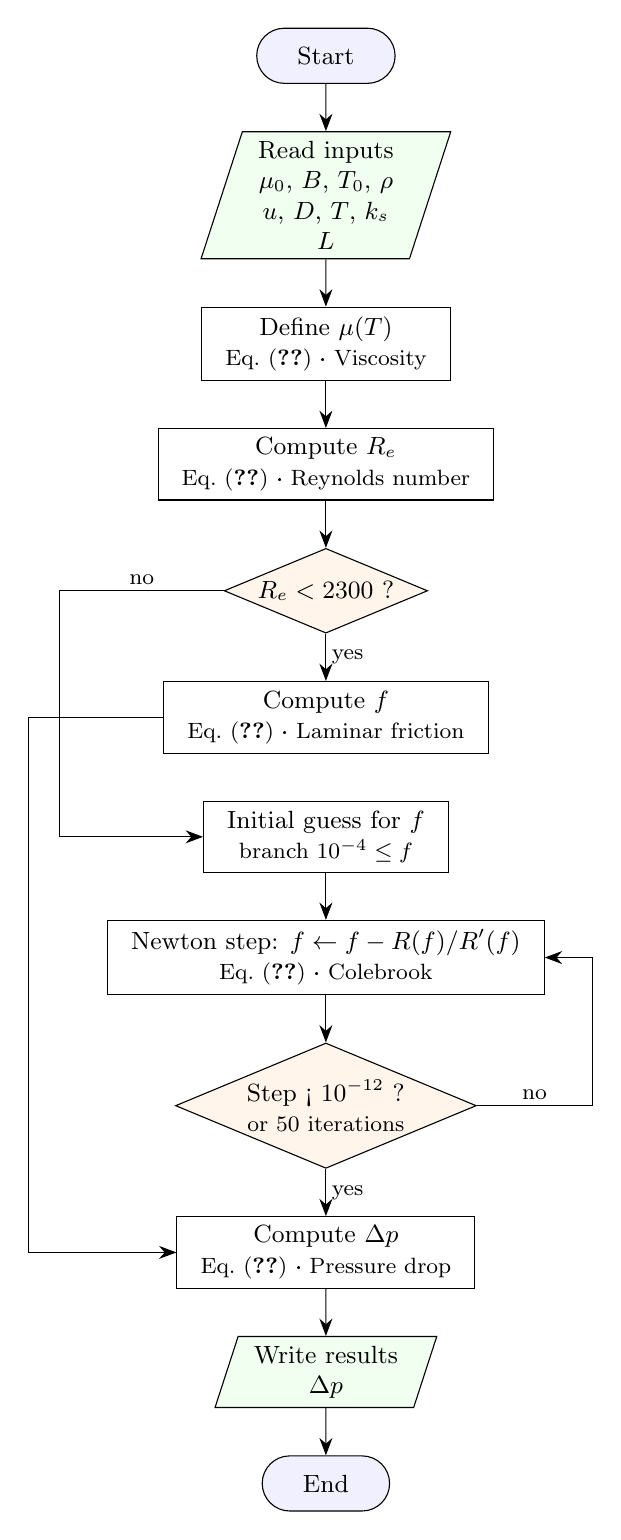
\begin{tikzpicture}[
  node distance=6mm, >={Stealth[length=2.2mm]}, font=\small,
  every node/.style={align=center},
  term/.style={draw, rounded rectangle, minimum height=7mm, inner xsep=5mm, fill=blue!6},
  io/.style={draw, trapezium, trapezium left angle=72, trapezium right angle=108, trapezium stretches body, minimum height=8mm, inner xsep=2mm, fill=green!6},
  proc/.style={draw, rectangle, minimum height=8mm, minimum width=30mm, inner xsep=3mm},
  dec/.style={draw, diamond, aspect=2.4, inner sep=1pt, fill=orange!8},
  lbl/.style={font=\footnotesize, inner sep=2pt}]
  \node[term] (n1) {Start};
  \node[io, below=of n1] (n2) {Read inputs \\ $\mu_0$, $B$, $T_0$, $\rho$ \\ $u$, $D$, $T$, $k_s$ \\ $L$};
  \node[proc, below=of n2] (n3) {Define $\mu(T)$ \\ {\footnotesize Eq.~\eqref{eq:viscosity} \textperiodcentered{} Viscosity}};
  \node[proc, below=of n3] (n4) {Compute $R_e$ \\ {\footnotesize Eq.~\eqref{eq:reynolds-number} \textperiodcentered{} Reynolds number}};
  \node[dec, below=of n4] (n5) {$R_e < 2300$ ?};
  \node[proc, below=of n5] (n6) {Compute $f$ \\ {\footnotesize Eq.~\eqref{eq:laminar-friction} \textperiodcentered{} Laminar friction}};
  \node[proc, below=of n6] (n7) {Initial guess for $f$ \\ {\footnotesize branch $10^{-4} \le f$}};
  \node[proc, below=of n7] (n8) {Newton step: $f \leftarrow f - R(f) / R'(f)$ \\ {\footnotesize Eq.~\eqref{eq:colebrook} \textperiodcentered{} Colebrook}};
  \node[dec, below=of n8] (n9) {Step < $10^{-12}$ ? \\ {\footnotesize or 50 iterations}};
  \node[proc, below=of n9] (n10) {Compute $\Delta p$ \\ {\footnotesize Eq.~\eqref{eq:pressure-drop} \textperiodcentered{} Pressure drop}};
  \node[io, below=of n10] (n11) {Write results \\ $\Delta p$};
  \node[term, below=of n11] (n12) {End};
  \coordinate (E) at (current bounding box.east);
  \coordinate (L0) at ([xshift=6mm]E);
  \draw[->] (n1) -- (n2);
  \draw[->] (n2) -- (n3);
  \draw[->] (n3) -- (n4);
  \draw[->] (n4) -- (n5);
  \draw[->] (n5) -- node[lbl, right] {yes} (n6);
  \draw[->] (n7) -- (n8);
  \draw[->] (n8) -- (n9);
  \draw[->] (n9) -- node[lbl, right] {yes} (n10);
  \draw[->] (n10) -- (n11);
  \draw[->] (n11) -- (n12);
  \draw[->] (n9.east) -- node[lbl, above] {no} (n9.east -| L0) |- (n8.east);
  \coordinate (W) at (current bounding box.west);
  \coordinate (J0) at ([xshift=-6mm]W);
  \coordinate (J1) at ([xshift=-10mm]W);
  \draw[->] (n5.west) -- node[lbl, above] {no} (n5.west -| J0) |- (n7.west);
  \draw[->] (n6.west) -- (n6.west -| J1) |- (n10.west);
\end{tikzpicture}
  \end{adjustbox}
  \caption{Flowchart of the solution procedure}\label{fig:flowchart}
\end{figure}

\end{document}